\chapter{Thiết kế Cơ sở dữ liệu Logic và Chuẩn hóa}

Chương này chuyển mô hình quan niệm sang mô hình quan hệ, xác định khóa và kiểm tra chuẩn hóa theo các phụ thuộc hàm đã nêu. Chuẩn hóa giúp hạn chế dị thường dữ liệu; không tự bảo đảm mọi quy tắc nghiệp vụ hoặc hiệu năng truy vấn.

\section{Chuyển đổi từ Mô hình Quan niệm sang Lược đồ Logic}

Dựa trên sơ đồ thực thể kết hợp (ERD) và các quy tắc nghiệp vụ đã phân tích ở Chương 2, tiến hành chuyển đổi mô hình thực thể quan niệm sang mô hình quan hệ (Relational Schema). Quá trình này được thực hiện thông qua việc áp dụng nghiêm ngặt các thuật toán ánh xạ ER sang quan hệ.

\subsection{Các quy tắc chuyển đổi áp dụng}
Quá trình ánh xạ từ ERD sang Lược đồ Logic tuân thủ các quy tắc cốt lõi sau:

\begin{itemize}
    \item \textbf{Quy tắc 1 (Ánh xạ Thực thể mạnh):} Mỗi thực thể (Entity) mạnh trong ERD được chuyển thành một quan hệ (Bảng - Table) trong Lược đồ Logic. Các thuộc tính đơn trở thành các cột (Columns) của bảng. Khóa định danh của thực thể trở thành Khóa chính (Primary Key - PK).
    
    \item \textbf{Quy tắc 2 (Ánh xạ mối kết hợp 1:N):} Đối với các mối kết hợp một-nhiều (ví dụ: \texttt{Merchant} - \texttt{Campaign}, \texttt{Customer} - \texttt{Credit}), đưa khóa chính của bảng phía "1" sang bảng phía "N" làm khóa ngoại (Foreign Key - FK).
    
    \item \textbf{Quy tắc 3 (Ánh xạ mối kết hợp M:N):} Tạo một quan hệ trung gian cho mối kết hợp nhiều-nhiều (ví dụ Customer và Merchant thông qua Credit). Đưa khóa của hai thực thể vào làm khóa ngoại. Trong CREDIT, chọn CreditID làm PK và đặt UNIQUE(CustomerID, MerchantID) cho khóa nghiệp vụ; không ghép CreditID vào cặp khóa này.
    \item \textbf{Quan hệ tự tham chiếu:} Đưa ManagerID nullable vào USER làm FK tham chiếu UserID, giữ nguyên quan hệ quản lý của ERD.
\end{itemize}

\subsection{Danh sách Lược đồ Quan hệ sơ bộ}
Dựa trên ERD của OctaPoint CaaS, áp dụng các quy tắc trên, ta thu được tập hợp các lược đồ quan hệ sơ bộ như sau. (Quy ước: Thuộc tính gạch chân là Khóa chính - PK, thuộc tính in nghiêng là Khóa ngoại - FK).

\begin{description}
    \item[\texttt{Tenant}] (\underline{TenantID}, TenantName, SystemConfig)
    \item[\texttt{Merchant}] (\underline{MerchantID}, \textit{TenantID}, BusinessName, Status)
    \item[\texttt{Role}] (\underline{RoleID}, RoleName)

    \item[\texttt{User}] (\underline{UserID}, \textit{MerchantID}, Email, PasswordHash, \textit{RoleID}, \textit{ManagerID})
    \item[\texttt{Campaign}] (\underline{CampaignID}, \textit{MerchantID}, CampaignName, StartDate, EndDate, Status)
    \item[\texttt{RewardRule}] (\underline{RuleID}, \textit{CampaignID}, ActionType, PointsMultiplier)
    \item[\texttt{User}] (\underline{UserID}, \textit{MerchantID}, Email, PasswordHash, \textit{RoleID}, \textit{ManagerID})    
    \item[\texttt{Campaign}] (\underline{CampaignID}, \textit{MerchantID}, CampaignName, StartDate, EndDate, Status)
    \item[\texttt{RewardRule}] (\underline{RuleID}, \textit{CampaignID}, ActionType, PointsMultiplier) 
    \item[\texttt{Customer}] (\underline{CustomerID}, WalletAddress, Email)
    \item[\texttt{Credit}] (\underline{CreditID}, \textit{CustomerID}, \textit{MerchantID}, AvailableBalance)
    \item[\texttt{CreditTransaction}] (\underline{TransactionID}, \textit{CreditID}, \textit{CampaignID}, Amount, TransactionType, SuiTxDigest, CreatedAt)
    \item[\texttt{APICredential}] (\underline{KeyID}, \textit{MerchantID}, ApiKey, SecretHash)
\end{description}

\section{Phụ thuộc hàm và Khóa ứng viên}

Phân tích được thực hiện trên từng quan hệ, không dùng tên thuộc tính trùng nhau ở nhiều bảng như một thuộc tính chung. Kết luận chuẩn hóa chỉ áp dụng cho tập phụ thuộc hàm nghiệp vụ được nêu dưới đây; việc dùng UUID không tự bảo đảm BCNF.

\subsection{Tập phụ thuộc hàm được xét}
Ký hiệu $R$ là toàn bộ thuộc tính của quan hệ tương ứng. Trong mỗi dòng dưới đây, từng vế trái liệt kê xác định mọi thuộc tính còn lại của $R$.
\begin{itemize}
    \item TENANT: TenantID $\rightarrow R$.
    \item MERCHANT: MerchantID $\rightarrow R$.
    \item ROLE: RoleID $\rightarrow R$.
    \item USER: UserID $\rightarrow R$; Email $\rightarrow R$, với $R$ gồm UserID, MerchantID, Email, PasswordHash, RoleID, ManagerID.
    \item CUSTOMER: CustomerID $\rightarrow R$.
    \item CAMPAIGN: CampaignID $\rightarrow R$.
    \item REWARD\_RULE: RuleID $\rightarrow R$.
    \item CREDIT: CreditID $\rightarrow R$; (CustomerID, MerchantID) $\rightarrow R$.
    \item API\_CREDENTIAL: KeyID $\rightarrow R$; ApiKey $\rightarrow R$.
    \item CREDIT\_TRANSACTION: TransactionID $\rightarrow R$, bao gồm cả CreatedAt.
\end{itemize}
Các khóa nghiệp vụ Email của USER, ApiKey và cặp (CustomerID, MerchantID) đều NOT NULL và UNIQUE. WalletAddress và SuiTxDigest chỉ duy nhất trên các dòng khác NULL; không coi chúng là khóa ứng viên của toàn quan hệ theo mô hình quan hệ cổ điển.

Không giả định RoleName, Customer.Email, CampaignName hoặc (CampaignID, ActionType) duy nhất. Không giả định MerchantID xác định RoleID hoặc ManagerID. Nếu bổ sung phụ thuộc hàm nghiệp vụ khác, cần kiểm tra chuẩn hóa lại.

\subsection{Bao đóng và tính tối thiểu}
Với USER, $\{UserID\}^{+}=R_{User}$ và $\{Email\}^{+}=R_{User}$. Không có phụ thuộc từ tập rỗng, nên cả hai tập đơn đều tối thiểu và là khóa ứng viên.

Với CREDIT, $\{CreditID\}^{+}=R_{Credit}$ và $\{CustomerID,MerchantID\}^{+}=R_{Credit}$. CustomerID riêng không xác định ví vì một khách có ví ở nhiều Merchant; MerchantID riêng không xác định ví vì một cửa hàng phục vụ nhiều khách. Do đó cặp là khóa ứng viên tối thiểu. CreditID được chọn làm PK để giao dịch tham chiếu gọn hơn; UNIQUE trên cặp vẫn bắt buộc.

Với API\_CREDENTIAL, KeyID và ApiKey là hai khóa ứng viên đơn, mỗi khóa có bao đóng bằng toàn quan hệ. Với các bảng còn lại, ID ở dòng tương ứng có bao đóng bằng toàn quan hệ và là khóa ứng viên đơn theo tập phụ thuộc hàm đã xét.

\section{Chuẩn hóa Dữ liệu}
Một quan hệ đạt BCNF nếu mọi phụ thuộc hàm không tầm thường $X \rightarrow Y$ có $X$ là siêu khóa. Trong tập phụ thuộc trên, tất cả vế trái đều là khóa ứng viên của chính quan hệ đó. Theo tập phụ thuộc này, mười quan hệ đáp ứng BCNF.

Kết luận này giảm dị thường cập nhật do các phụ thuộc hàm đã xét, không thay thế ràng buộc miền giá trị, kiểm soát đồng thời hoặc toàn vẹn liên bảng. AvailableBalance là số dư lưu sẵn để tra cứu; phải được tầng dịch vụ duy trì nhất quán với sổ cái, không thể suy ra tính nhất quán đó chỉ từ BCNF.


\subsection{Cách kiểm tra dạng chuẩn}
1NF yêu cầu mỗi ô chứa một giá trị thuộc miền đã chọn, không chứa danh sách lặp. 2NF yêu cầu đạt 1NF và thuộc tính không khóa không phụ thuộc vào một phần thực sự của khóa ứng viên. 3NF yêu cầu với mỗi phụ thuộc hàm không tầm thường, vế trái là siêu khóa hoặc thuộc tính vế phải là thuộc tính khóa. BCNF yêu cầu vế trái luôn là siêu khóa.

Ví dụ, nếu đưa TenantName vào MERCHANT thì xuất hiện MerchantID xác định TenantID và TenantID xác định TenantName. Một tổ chức có nhiều cửa hàng sẽ khiến tên tổ chức bị lưu lặp. Giữ TenantName ở TENANT và tham chiếu bằng TenantID giúp tránh cập nhật tên ở nhiều dòng MERCHANT.

\section{Sơ đồ Lược đồ Logic (Logical Schema Diagram)}

Lược đồ dưới đây tương ứng với tập phụ thuộc hàm đã xét ở mục chuẩn hóa. Các ràng buộc miền giá trị và duy nhất bổ sung được trình bày ở từ điển dữ liệu.

Đặc biệt, hệ thống tồn tại mối kết hợp Nhiều - Nhiều (M:N) giữa \texttt{CUSTOMER} và \texttt{MERCHANT}. Mối kết hợp này đã được phân rã thành hai mối quan hệ 1-N thông qua thực thể trung gian (Associative Entity) là bảng \texttt{CREDIT}.

Dưới đây là Sơ đồ Logic thể hiện trực quan cấu trúc các bảng, tập hợp đầy đủ các thuộc tính, khóa chính (Primary Key - PK) và các mối quan hệ khóa ngoại (Foreign Key - FK) kèm bản số (1-N) liên kết giữa các bảng.

\begin{figure}[H]
    \centering
    \resizebox{\textwidth}{!}{ % Co theo chieu rong trang
    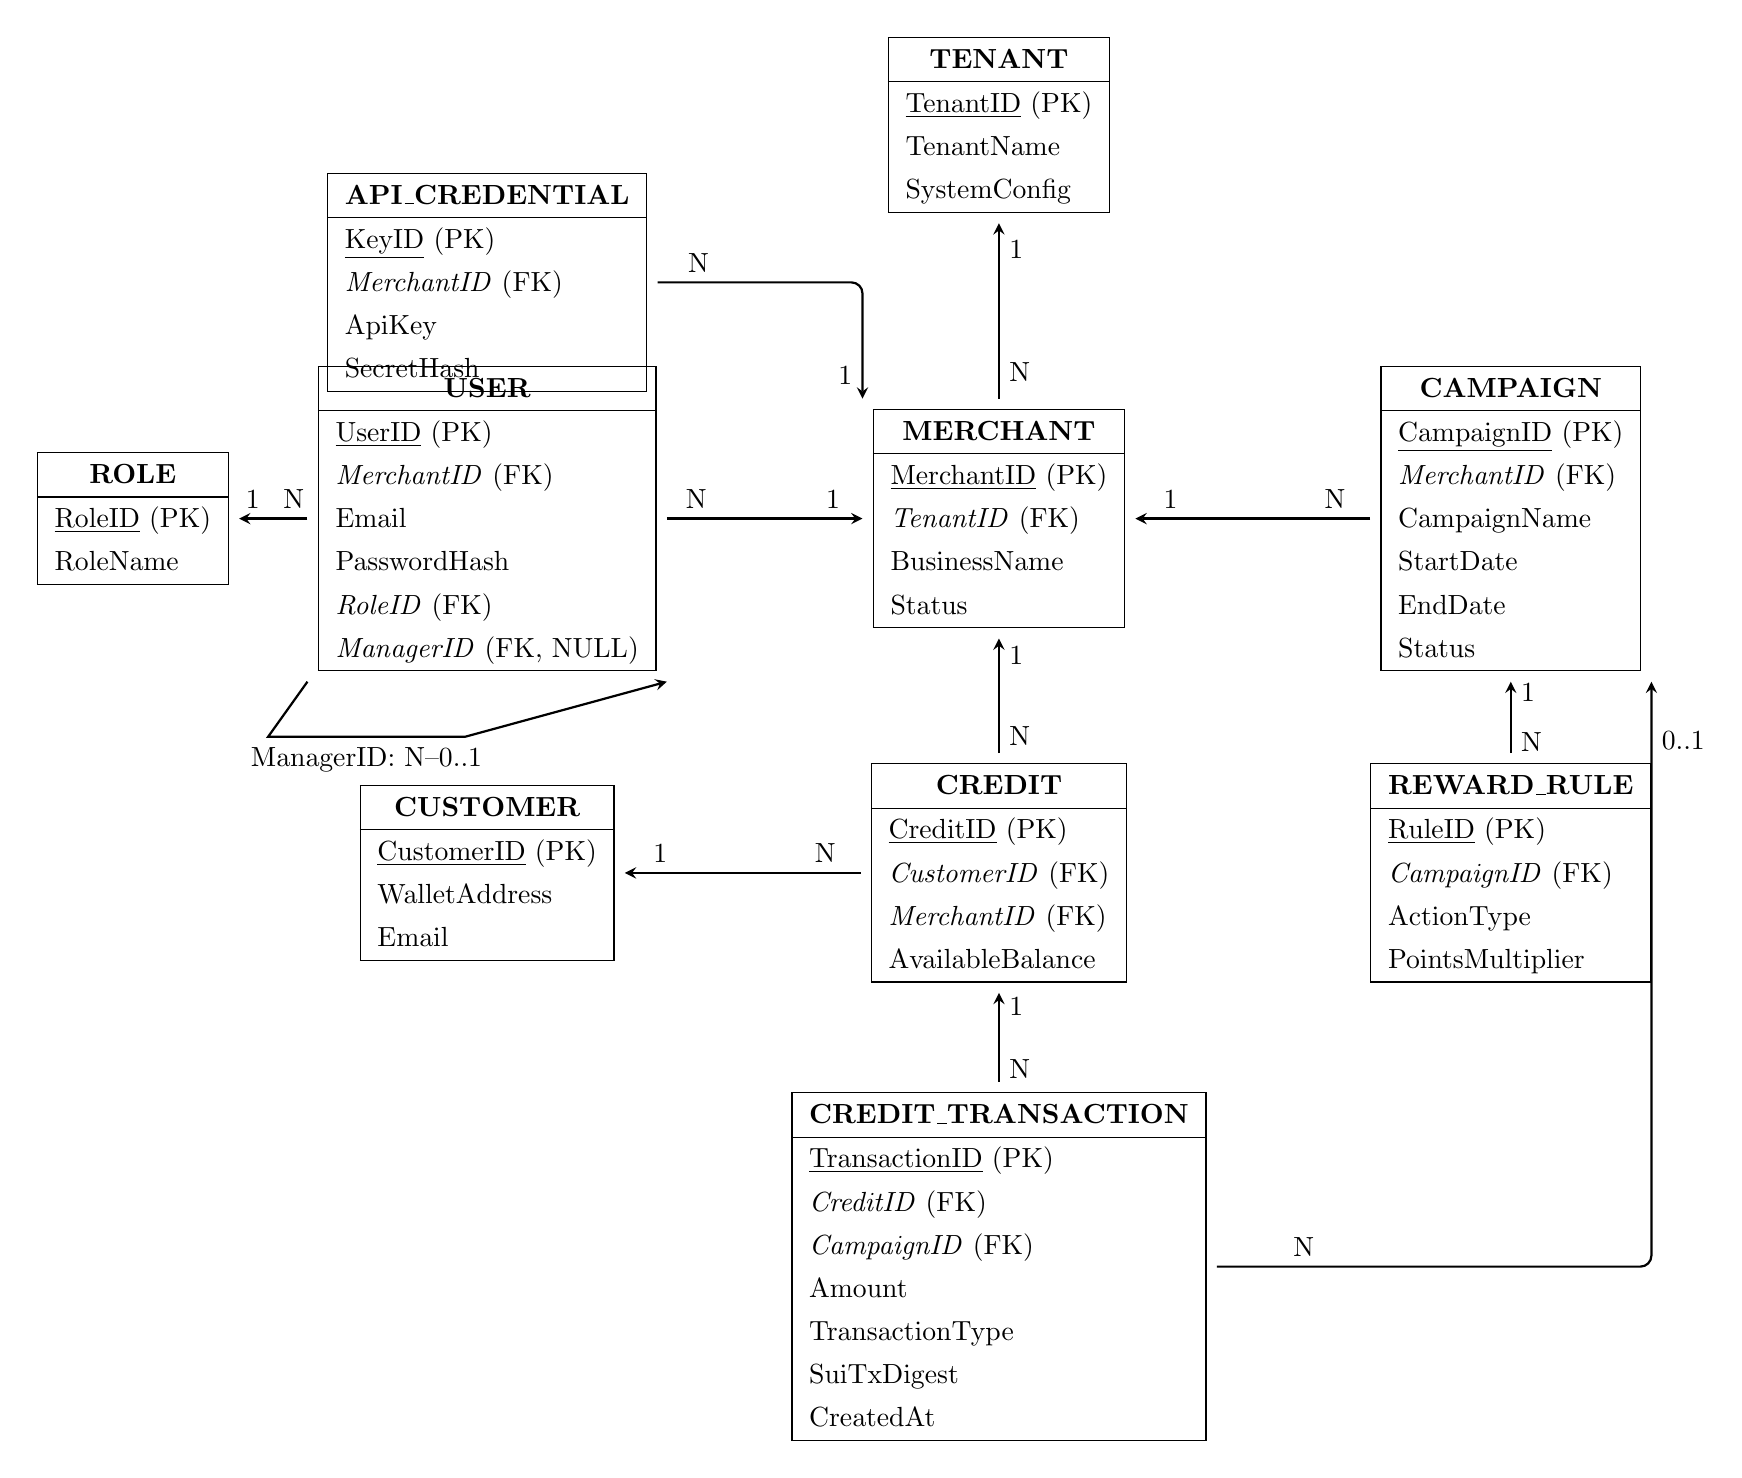
\begin{tikzpicture}[>=stealth, thick]

        % Bảng TENANT
        \node (tenant) at (0, 6.5) {
            \begin{tabular}{|l|}
            \hline
            \multicolumn{1}{|c|}{\textbf{TENANT}} \\ \hline
            \underline{TenantID} (PK) \\
            TenantName \\
            SystemConfig \\ \hline
            \end{tabular}
        };

        % Bảng MERCHANT
        \node (merchant) at (0, 1.5) {
            \begin{tabular}{|l|}
            \hline
            \multicolumn{1}{|c|}{\textbf{MERCHANT}} \\ \hline
            \underline{MerchantID} (PK) \\
            \textit{TenantID} (FK) \\
            BusinessName \\
            Status \\ \hline
            \end{tabular}
        };

        % Bảng API_CREDENTIAL (Đã bổ sung)
        \node (api) at (-6.5, 4.5) {
            \begin{tabular}{|l|}
            \hline
            \multicolumn{1}{|c|}{\textbf{API\_CREDENTIAL}} \\ \hline
            \underline{KeyID} (PK) \\
            \textit{MerchantID} (FK) \\
            ApiKey \\
            SecretHash \\ \hline
            \end{tabular}
        };

        % Bảng USER
        \node (user) at (-6.5, 1.5) {
            \begin{tabular}{|l|}
            \hline
            \multicolumn{1}{|c|}{\textbf{USER}} \\ \hline
            \underline{UserID} (PK) \\
            \textit{MerchantID} (FK) \\
            Email \\
            PasswordHash \\
            \textit{RoleID} (FK) \\
            \textit{ManagerID} (FK, NULL) \\ \hline
            \end{tabular}
        };

        % Bang ROLE va quan he quan ly tu tham chieu
        \node (role) at (-11, 1.5) {
            \begin{tabular}{|l|}
            \hline
            \multicolumn{1}{|c|}{\textbf{ROLE}} \\ \hline
            \underline{RoleID} (PK) \\
            RoleName \\ \hline
            \end{tabular}
        };
        \draw[->] (user.west) -- node[pos=0.2, above] {N} node[pos=0.8, above] {1} (role.east);
        \draw[->] (user.south west) -- ++(-0.5,-0.7) -- ++(2.5,0)
            node[midway, below] {ManagerID: N--0..1} -- (user.south east);

        % Bảng CAMPAIGN
        \node (campaign) at (6.5, 1.5) {
            \begin{tabular}{|l|}
            \hline
            \multicolumn{1}{|c|}{\textbf{CAMPAIGN}} \\ \hline
            \underline{CampaignID} (PK) \\
            \textit{MerchantID} (FK) \\
            CampaignName \\
            StartDate \\
            EndDate \\
            Status \\ \hline
            \end{tabular}
        };

        % Bảng CUSTOMER
        \node (customer) at (-6.5, -3) {
            \begin{tabular}{|l|}
            \hline
            \multicolumn{1}{|c|}{\textbf{CUSTOMER}} \\ \hline
            \underline{CustomerID} (PK) \\
            WalletAddress \\
            Email \\ \hline
            \end{tabular}
        };

        % Bảng CREDIT (Bảng trung gian giải quyết quan hệ N-N)
        \node (credit) at (0, -3) {
            \begin{tabular}{|l|}
            \hline
            \multicolumn{1}{|c|}{\textbf{CREDIT}} \\ \hline
            \underline{CreditID} (PK) \\
            \textit{CustomerID} (FK) \\
            \textit{MerchantID} (FK) \\
            AvailableBalance \\ \hline
            \end{tabular}
        };

        % Bảng REWARD_RULE
        \node (rule) at (6.5, -3) {
            \begin{tabular}{|l|}
            \hline
            \multicolumn{1}{|c|}{\textbf{REWARD\_RULE}} \\ \hline
            \underline{RuleID} (PK) \\
            \textit{CampaignID} (FK) \\
            ActionType \\
            PointsMultiplier \\ \hline
            \end{tabular}
        };

        % Bảng CREDIT_TRANSACTION
        \node (transaction) at (0, -8) {
            \begin{tabular}{|l|}
            \hline
            \multicolumn{1}{|c|}{\textbf{CREDIT\_TRANSACTION}} \\ \hline
            \underline{TransactionID} (PK) \\
            \textit{CreditID} (FK) \\
            \textit{CampaignID} (FK) \\
            Amount \\
            TransactionType \\
            SuiTxDigest \\
            CreatedAt \\ \hline
            \end{tabular}
        };

        % ========================================================
        % VẼ DÂY NỐI CÓ GẮN NHÃN BẢN SỐ (1 và N)
        % ========================================================
        
        % MERCHANT -> TENANT
        \draw[->] (merchant.north) -- node[pos=0.15, right] {N} node[pos=0.85, right] {1} (tenant.south);
        
        % API -> MERCHANT (Dây gấp khúc)
        \draw[->, rounded corners] (api.east) -| node[pos=0.1, above] {N} node[pos=0.9, left] {1} (merchant.north west);
        
        % USER -> MERCHANT
        \draw[->] (user.east) -- node[pos=0.15, above] {N} node[pos=0.85, above] {1} (merchant.west);
        
        % CAMPAIGN -> MERCHANT
        \draw[->] (campaign.west) -- node[pos=0.15, above] {N} node[pos=0.85, above] {1} (merchant.east);
        
        % CREDIT -> MERCHANT
        \draw[->] (credit.north) -- node[pos=0.15, right] {N} node[pos=0.85, right] {1} (merchant.south);
        
        % CREDIT -> CUSTOMER
        \draw[->] (credit.west) -- node[pos=0.15, above] {N} node[pos=0.85, above] {1} (customer.east);
        
        % REWARD_RULE -> CAMPAIGN
        \draw[->] (rule.north) -- node[pos=0.15, right] {N} node[pos=0.85, right] {1} (campaign.south);
        
        % TRANSACTION -> CREDIT
        \draw[->] (transaction.north) -- node[pos=0.15, right] {N} node[pos=0.85, right] {1} (credit.south);
        
        % TRANSACTION -> CAMPAIGN (Dây gấp khúc vòng lên)
        \draw[->, rounded corners] (transaction.east) -| node[pos=0.1, above] {N} node[pos=0.95, right] {0..1} (campaign.south east);

    \end{tikzpicture}
    }
    \caption{Sơ đồ Lược đồ Logic chi tiết hệ thống OctaPoint CaaS}
    \label{fig:sodo_logic_tikz}
\end{figure}

\textit{Ghi chú:} Sơ đồ thể hiện rõ việc phân rã mối kết hợp N-N giữa Khách hàng và Doanh nghiệp thông qua thực thể trung gian \texttt{CREDIT}. Các đường liên kết chỉ hướng tham chiếu từ Khóa ngoại (nhánh N) trỏ tới Khóa chính (nhánh 1), đảm bảo chặt chẽ ràng buộc toàn vẹn tham chiếu.
Mỗi cặp (CustomerID, MerchantID) ở CREDIT có tối đa một bản ghi. Nhãn N chỉ số lượng tối đa ở phía tham chiếu; RoleID bắt buộc, ManagerID và CampaignID của giao dịch tùy chọn.

\section{Từ điển Dữ liệu (Data Dictionary)}

Từ điển dữ liệu (Data Dictionary) mô tả chi tiết cấu trúc vật lý của các bảng trong cơ sở dữ liệu. Nó bao gồm tên các thuộc tính, kiểu dữ liệu, các ràng buộc toàn vẹn (Khóa chính - PK, Khóa ngoại - FK, Not Null) và diễn giải ý nghĩa của từng trường dữ liệu để chuẩn bị cho bước triển khai vật lý ở Chương 4.

\subsection{Bảng TENANT (Đơn vị thuê bao)}
Lưu trữ thông tin về các đơn vị khách hàng lớn thuê hệ thống OctaPoint CaaS.

\begin{table}[H]
    \centering
    \renewcommand{\arraystretch}{1.3}
    \begin{tabularx}{\textwidth}{|>{\raggedright\arraybackslash}p{3cm}|>{\raggedright\arraybackslash}p{2.8cm}|>{\raggedright\arraybackslash}p{2cm}|>{\raggedright\arraybackslash}X|}
        \hline
        \textbf{Tên thuộc tính} & \textbf{Kiểu dữ liệu} & \textbf{Ràng buộc} & \textbf{Mô tả} \\ \hline
        TenantID & VARCHAR(36) & PK, NOT NULL & Mã định danh duy nhất (UUID). \\ \hline
        TenantName & NVARCHAR(255) & NOT NULL & Tên định danh của đơn vị thuê bao. \\ \hline
        SystemConfig & NVARCHAR(MAX) & NULL, CHECK & Cấu hình hệ thống riêng của Tenant. \\ \hline
    \end{tabularx}
\end{table}

\subsection{Bảng MERCHANT (Doanh nghiệp đối tác)}
Lưu trữ thông tin các doanh nghiệp/cửa hàng trực thuộc một Tenant.

\begin{table}[H]
    \centering
    \renewcommand{\arraystretch}{1.3}
    \begin{tabularx}{\textwidth}{|>{\raggedright\arraybackslash}p{3cm}|>{\raggedright\arraybackslash}p{2.8cm}|>{\raggedright\arraybackslash}p{2cm}|>{\raggedright\arraybackslash}X|}
        \hline
        \textbf{Tên thuộc tính} & \textbf{Kiểu dữ liệu} & \textbf{Ràng buộc} & \textbf{Mô tả} \\ \hline
        MerchantID & VARCHAR(36) & PK, NOT NULL & Mã định danh duy nhất của Merchant. \\ \hline
        TenantID & VARCHAR(36) & FK, NOT NULL & Tham chiếu đến bảng TENANT. \\ \hline
        BusinessName & NVARCHAR(255) & NOT NULL & Tên thương hiệu/doanh nghiệp. \\ \hline
        Status & VARCHAR(20) & NOT NULL & Trạng thái hoạt động (Active, Suspended). \\ \hline
    \end{tabularx}
\end{table}

\subsection{Bảng USER (Tài khoản nhân sự)}
Quản lý tài khoản đăng nhập của nhân viên thuộc các Merchant.

\begin{table}[H]
    \centering
    \renewcommand{\arraystretch}{1.3}
    \begin{tabularx}{\textwidth}{|>{\raggedright\arraybackslash}p{3cm}|>{\raggedright\arraybackslash}p{2.8cm}|>{\raggedright\arraybackslash}p{2cm}|>{\raggedright\arraybackslash}X|}
        \hline
        \textbf{Tên thuộc tính} & \textbf{Kiểu dữ liệu} & \textbf{Ràng buộc} & \textbf{Mô tả} \\ \hline
        UserID & VARCHAR(36) & PK, NOT NULL & Mã định danh tài khoản. \\ \hline
        MerchantID & VARCHAR(36) & FK, NOT NULL & Tham chiếu đến bảng MERCHANT. \\ \hline
        Email & VARCHAR(255) & UNIQUE, NOT NULL & Email đăng nhập (duy nhất). \\ \hline
        PasswordHash & VARCHAR(255) & NOT NULL & Chuỗi băm mật khẩu bảo mật. \\ \hline
        RoleID & INT & FK, NOT NULL & Mã quyền hạn của người dùng. \\ \hline
        ManagerID & VARCHAR(36) & FK, NULL & Mã người quản lý trực tiếp (tham chiếu đến UserID). \\ \hline
    \end{tabularx}
\end{table}

\subsubsection{Bảng ROLE (Vai trò)}
Lưu trữ thông tin các nhóm quyền hạn để phân quyền người dùng trong hệ thống.

\begin{table}[H]
\centering
\begin{tabularx}{\textwidth}{|>{\raggedright\arraybackslash}p{3cm}|>{\raggedright\arraybackslash}p{2.8cm}|>{\raggedright\arraybackslash}p{2cm}|>{\raggedright\arraybackslash}X|}
\hline
\textbf{Tên thuộc tính} & \textbf{Kiểu dữ liệu} & \textbf{Ràng buộc} & \textbf{Mô tả} \\ \hline
RoleID & INT & PK, NOT NULL & Mã định danh vai trò. \\ \hline
RoleName & NVARCHAR(50) & NOT NULL & Tên hiển thị của vai trò (VD: Admin, Staff). \\ \hline
\end{tabularx}
\end{table}

\subsection{Bảng CUSTOMER (Khách hàng)}
Quản lý thông tin định danh của khách hàng tích điểm.

\begin{table}[H]
    \centering
    \renewcommand{\arraystretch}{1.3}
    \begin{tabularx}{\textwidth}{|>{\raggedright\arraybackslash}p{3cm}|>{\raggedright\arraybackslash}p{2.8cm}|>{\raggedright\arraybackslash}p{2cm}|>{\raggedright\arraybackslash}X|}
        \hline
        \textbf{Tên thuộc tính} & \textbf{Kiểu dữ liệu} & \textbf{Ràng buộc} & \textbf{Mô tả} \\ \hline
        CustomerID & VARCHAR(36) & PK, NOT NULL & Mã định danh khách hàng nội bộ. \\ \hline
        WalletAddress & VARCHAR(100) & UNIQUE*, NULL & Địa chỉ ví blockchain (Sui) dùng cho Walletless Auth. \\ \hline
        Email & VARCHAR(255) & NULL & Địa chỉ email (Định danh Web2). \\ \hline
    \end{tabularx}
\end{table}

\subsection{Bảng CAMPAIGN (Chiến dịch)}
Quản lý các chương trình khuyến mãi, tích/đổi điểm.

\begin{table}[H]
    \centering
    \renewcommand{\arraystretch}{1.3}
    \begin{tabularx}{\textwidth}{|>{\raggedright\arraybackslash}p{3cm}|>{\raggedright\arraybackslash}p{2.8cm}|>{\raggedright\arraybackslash}p{2cm}|>{\raggedright\arraybackslash}X|}
        \hline
        \textbf{Tên thuộc tính} & \textbf{Kiểu dữ liệu} & \textbf{Ràng buộc} & \textbf{Mô tả} \\ \hline
        CampaignID & VARCHAR(36) & PK, NOT NULL & Mã định danh chiến dịch. \\ \hline
        MerchantID & VARCHAR(36) & FK, NOT NULL & Tham chiếu đến bảng MERCHANT. \\ \hline
        CampaignName & NVARCHAR(255) & NOT NULL & Tên chiến dịch. \\ \hline
        StartDate & DATETIME & NOT NULL & Thời gian bắt đầu. \\ \hline
        EndDate & DATETIME & NULL & Thời điểm kết thúc (NULL nếu vô thời hạn). \\ \hline
        Status & VARCHAR(20) & NOT NULL & Trạng thái (Draft, Active, Expired). \\ \hline
    \end{tabularx}
\end{table}

\subsection{Bảng CREDIT\_TRANSACTION (Sổ cái giao dịch điểm)}
Lưu vết toàn bộ các giao dịch cộng/trừ điểm thưởng, có lưu băm trên blockchain.

\begin{table}[H]
    \centering
    \renewcommand{\arraystretch}{1.3}
    \begin{tabularx}{\textwidth}{|>{\raggedright\arraybackslash}p{3cm}|>{\raggedright\arraybackslash}p{2.8cm}|>{\raggedright\arraybackslash}p{2cm}|>{\raggedright\arraybackslash}X|}
        \hline
        \textbf{Tên thuộc tính} & \textbf{Kiểu dữ liệu} & \textbf{Ràng buộc} & \textbf{Mô tả} \\ \hline
        TransactionID & VARCHAR(36) & PK, NOT NULL & Mã giao dịch định danh. \\ \hline
        CreditID & VARCHAR(36) & FK, NOT NULL & Tham chiếu đến ví điểm. \\ \hline
        CampaignID & VARCHAR(36) & FK, NULL & Tham chiếu đến chiến dịch. \\ \hline
        Amount & DECIMAL(18,2) & NOT NULL & Biến động có dấu: Earn $>0$, Redeem $<0$, Refund khác 0. \\ \hline
        TransactionType & VARCHAR(50) & NOT NULL & Loại giao dịch (Earn, Redeem, Refund). \\ \hline
        SuiTxDigest & VARCHAR(100) & UNIQUE*, NULL & Mã băm giao dịch trên mạng lưới Sui. \\ \hline
        CreatedAt & DATETIME & NOT NULL & Thời gian phát sinh giao dịch. \\ \hline
    \end{tabularx}
\end{table}

\subsection{Bảng CREDIT}
\begin{table}[H]
\centering
\small
\begin{tabularx}{\textwidth}{|>{\raggedright\arraybackslash}p{3cm}|>{\raggedright\arraybackslash}p{2.8cm}|>{\raggedright\arraybackslash}p{2cm}|>{\raggedright\arraybackslash}X|}
\hline
Thuộc tính & Kiểu dữ liệu & Ràng buộc & Mô tả \\ \hline
CreditID & VARCHAR(36) & PK, NOT NULL & Định danh ví. \\ \hline
CustomerID & VARCHAR(36) & FK, NOT NULL & Tham chiếu CUSTOMER. \\ \hline
MerchantID & VARCHAR(36) & FK, NOT NULL & Tham chiếu MERCHANT. \\ \hline
AvailableBalance & DECIMAL(18,2) & NOT NULL, CHECK & Số dư không âm, mặc định 0. \\ \hline
\end{tabularx}
\end{table}
\subsection{Bảng REWARD\_RULE}
\begin{table}[H]
\centering
\small
\begin{tabularx}{\textwidth}{|>{\raggedright\arraybackslash}p{3cm}|>{\raggedright\arraybackslash}p{2.8cm}|>{\raggedright\arraybackslash}p{2cm}|>{\raggedright\arraybackslash}X|}
\hline
Thuộc tính & Kiểu dữ liệu & Ràng buộc & Mô tả \\ \hline
RuleID & VARCHAR(36) & PK, NOT NULL & Định danh quy tắc. \\ \hline
CampaignID & VARCHAR(36) & FK, NOT NULL & Tham chiếu CAMPAIGN. \\ \hline
ActionType & VARCHAR(50) & NOT NULL & Mã hành động mở rộng, ví dụ Purchase, Birthday. \\ \hline
PointsMultiplier & DECIMAL(5,2) & NOT NULL, CHECK & Hệ số lớn hơn 0. \\ \hline
\end{tabularx}
\end{table}
\subsection{Bảng API\_CREDENTIAL}
\begin{table}[H]
\centering
\small
\begin{tabularx}{\textwidth}{|>{\raggedright\arraybackslash}p{3cm}|>{\raggedright\arraybackslash}p{2.8cm}|>{\raggedright\arraybackslash}p{2cm}|>{\raggedright\arraybackslash}X|}
\hline
Thuộc tính & Kiểu dữ liệu & Ràng buộc & Mô tả \\ \hline
KeyID & VARCHAR(36) & PK, NOT NULL & Định danh bản ghi khóa. \\ \hline
MerchantID & VARCHAR(36) & FK, NOT NULL & Tham chiếu MERCHANT. \\ \hline
ApiKey & VARCHAR(255) & UNIQUE, NOT NULL & Mã khóa công khai duy nhất. \\ \hline
SecretHash & VARCHAR(255) & NOT NULL & Giá trị băm của secret. \\ \hline
\end{tabularx}
\end{table}

\textit{Ràng buộc bổ sung:} UNIQUE* nghĩa là duy nhất khi khác NULL, được triển khai bằng chỉ mục có điều kiện. CREDIT có UNIQUE(CustomerID, MerchantID). EndDate phải không trước StartDate khi có giá trị; các miền Status và TransactionType có CHECK. SystemConfig phải là JSON object/array hợp lệ khi khác NULL. CreatedAt mặc định GETDATE(). ManagerID tham chiếu USER và không bằng UserID của chính dòng. Nội dung đầy đủ nằm trong \texttt{database/schema.sql}.

